%! Author = maxx
%! Date = 01/20/2025

% Preamble
\documentclass[12pt]{report}

\usepackage[a4paper, left=2.5cm, right=2.5cm, top=3cm, bottom=3cm]{geometry}
\usepackage{graphicx}
\usepackage{pdfpages}
\usepackage{glossaries}
\usepackage{titling}
\setlength{\parindent}{0pt}

\title{POO - Laboratoire 9 \\ \large Application de Dessin de Disques}
\author{Lestiboudois Maxime \& Parisod Nathan}
\date{20/01/2025}

% Redéfinir \maketitle pour inclure l'image sous le titre
\pretitle{\begin{center}\Huge\bfseries}
\posttitle{\par\end{center}\vspace{0.5cm}
\begin{center}
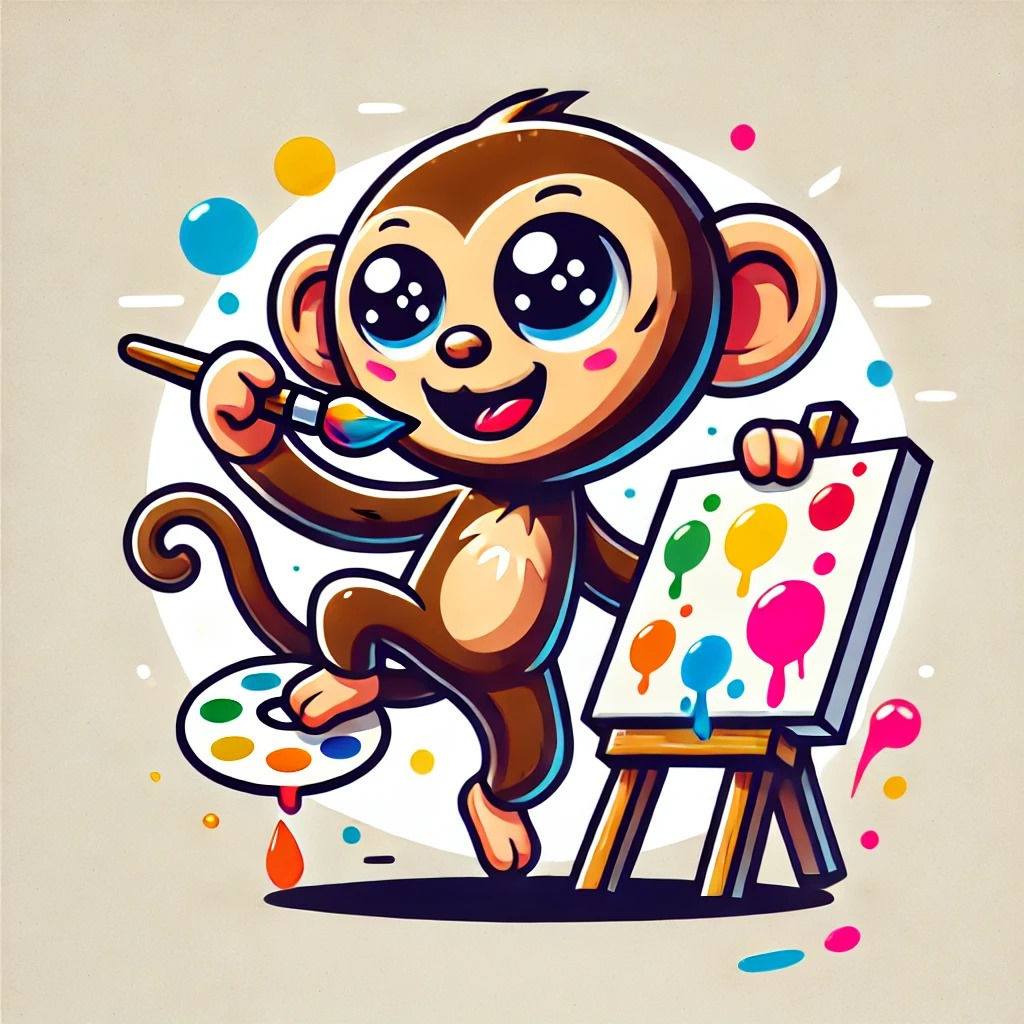
\includegraphics[scale = 0.4]{images/POO_Singe_ColoredPoint}
\end{center}\vspace{0.5cm}}

% Document
\begin{document}
    \maketitle
    \tableofcontents
    \newpage

%%%%%%%%%%%%%%%%%%%%
%%  Introduction  %%
%%%%%%%%%%%%%%%%%%%%

    \section*{Introduction}
    \addcontentsline{toc}{section}{Introduction}
    Ce laboratoire porte sur la création d'une application graphique interactive permettant de dessiner et manipuler des disques à l'aide de l'API Swing en Java.
    L'objectif principal est de mettre en pratique les concepts de programmation orientée objet et de gestion d'événements.

    Le projet implémente les fonctionnalités suivantes :
    \begin{itemize}
        \item Dessiner des disques en cliquant et en relâchant le bouton gauche de la souris.
        \item Effacer un disque en cliquant avec le bouton droit.
        \item Déplacer un disque en maintenant la touche SHIFT tout en cliquant et en déplaçant la souris.
        \item Réinitialiser le canvas avec un bouton "Clear".
        \item Quitter l'application avec un bouton "Quit".
    \end{itemize}

%%%%%%%%%%%%%%%%%%%%
%Cahier des charges%
%%%%%%%%%%%%%%%%%%%%
    \section*{Cahier des charges}
    \addcontentsline{toc}{section}{Cahier des charges}
    \subsection*{Objectif du Projet}
    \addcontentsline{toc}{subsection}{Objectif du Projet}
    Développer une application graphique interactive pour dessiner et manipuler des disques en suivant une architecture orientée objet.

    \subsection*{Spécifications Fonctionnelles}
    \addcontentsline{toc}{subsection}{Spécifications Fonctionnelles}
    \begin{itemize}
        \item Créer un disque avec le bouton gauche de la souris :
        \begin{itemize}
            \item Le centre du disque est défini par l'emplacement du clic.
            \item Le rayon est défini par la distance entre le clic initial et le relâchement de la souris.
        \end{itemize}
        \item Effacer un disque avec le bouton droit.
        \item Déplacer un disque en maintenant la touche SHIFT et en effectuant un glisser-déposer.
        \item Afficher un aperçu du disque en cours de création avant le relâchement de la souris.
        \item Boutons fonctionnels :
        \begin{itemize}
            \item Clear : réinitialise l'application.
            \item Quit : ferme l'application.
        \end{itemize}
    \end{itemize}

%%%%%%%%%%%%%%%%%%%%
%%  Schéma UML  %%
%%%%%%%%%%%%%%%%%%%%
    \section*{Schéma UML}
    \addcontentsline{toc}{section}{Schéma UML}
    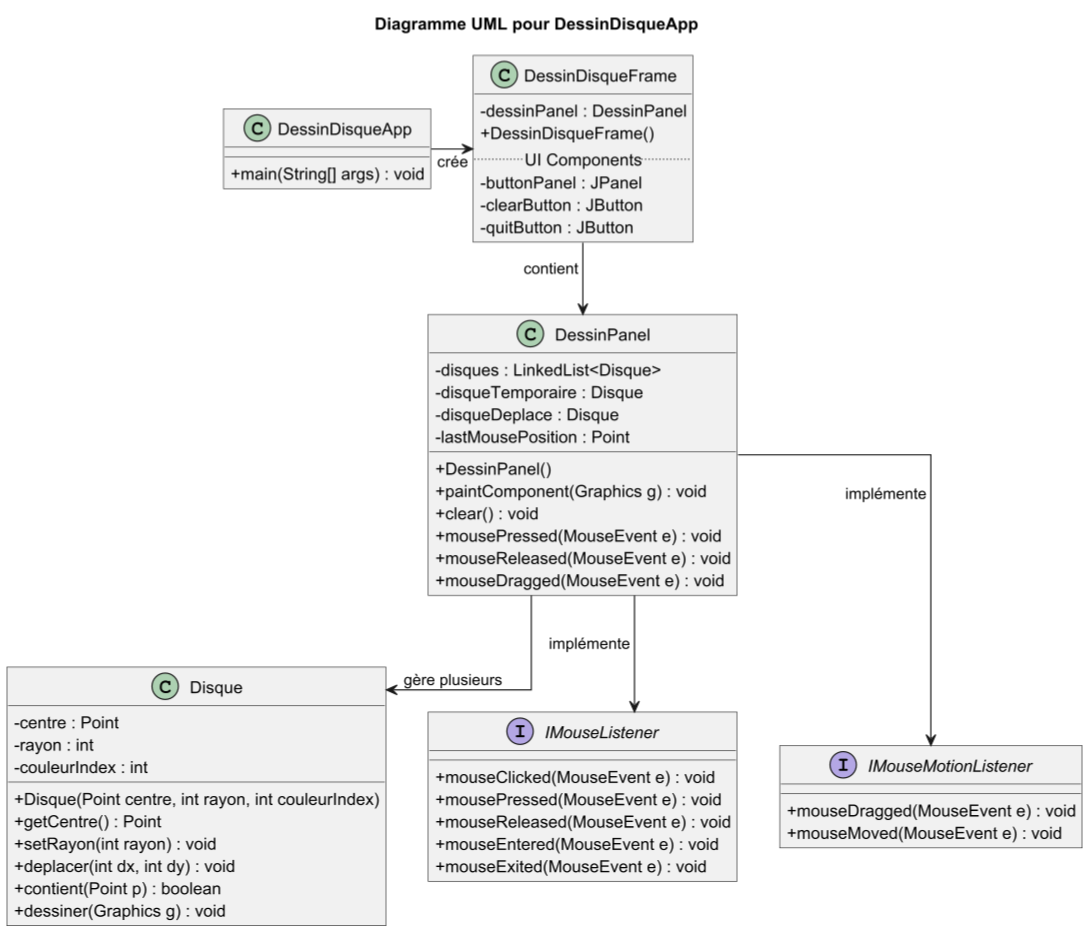
\includegraphics[scale=0.5]{images/SchemaUML}

%%%%%%%%%%%%%%%%%%%%
%%  Listing code  %%
%%%%%%%%%%%%%%%%%%%%
    \section*{Listing du code}
    \addcontentsline{toc}{section}{Listing du code}
    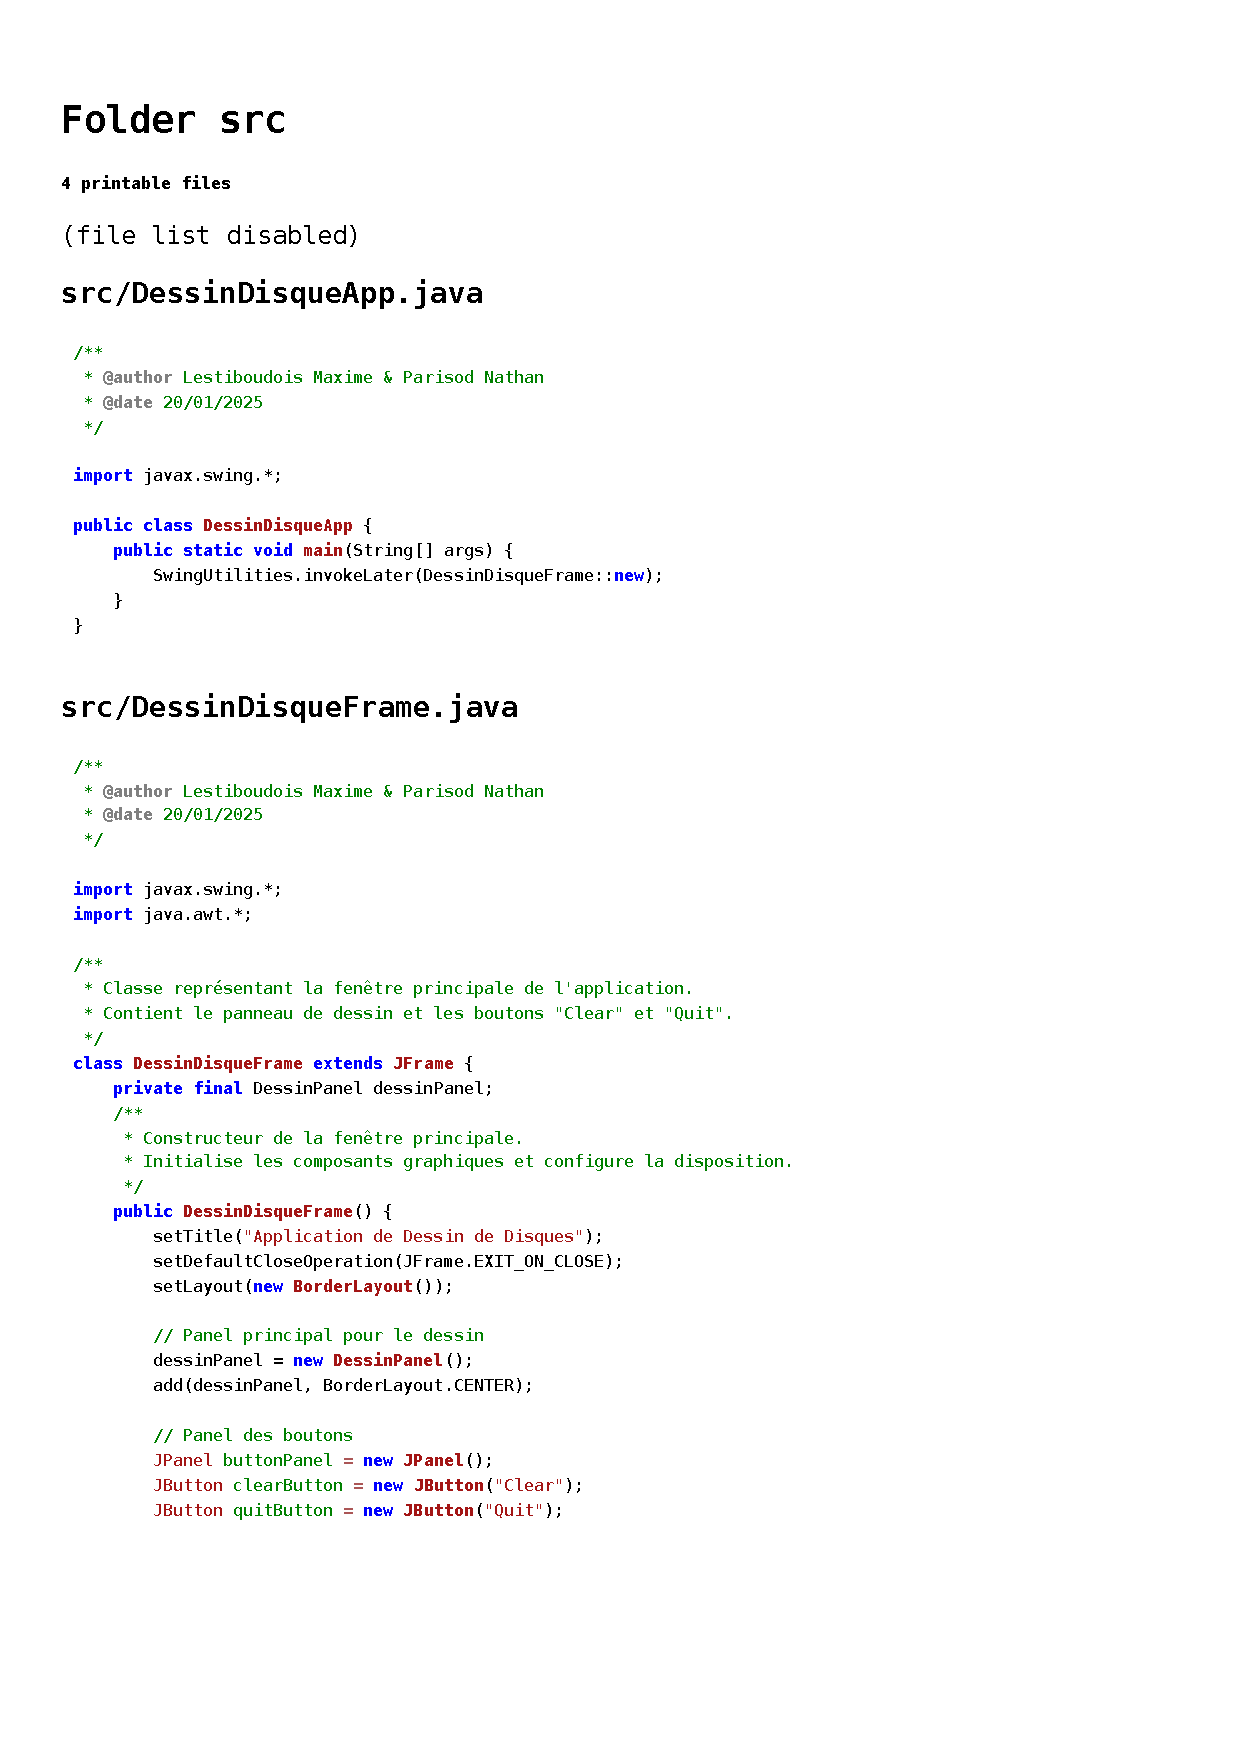
\includepdf[page=-, pagecommand={\thispagestyle{plain}}]{src.pdf}

%%%%%%%%%%%%%%%%%%%%
% Choix Conception %
%%%%%%%%%%%%%%%%%%%%
    \section*{Choix de conception}
    \addcontentsline{toc}{section}{Choix de conception}
    \subsection*{Structure orientée objet}
    \addcontentsline{toc}{subsection}{Structure orientée objet}
    L'application suit un modèle orienté objet pour garantir la modularité et la maintenabilité. Les principales classes incluent :
    \begin{itemize}
        \item \textbf{DessinDisquesApp} : classe principale lançant l'application.
        \item \textbf{DessinDisquesFrame} : fenêtre principale contenant les panneaux d'interaction.
        \item \textbf{DessinPanel} : panneau où les disques sont dessinés et manipulés.
        \item \textbf{Disque} : représente un disque avec son centre, son rayon et sa couleur.
    \end{itemize}

    \subsection*{Gestion des événements}
    \addcontentsline{toc}{subsection}{Gestion des événements}
    Les interactions utilisateur sont gérées via les interfaces \textbf{MouseListener} et \textbf{MouseMotionListener}, enregistrées sur le \textbf{DessinPanel}. Ces interfaces permettent de gérer :
    \begin{itemize}
        \item La création de disques.
        \item La suppression de disques.
        \item Le déplacement des disques avec SHIFT + clic gauche.
    \end{itemize}

    \subsection*{Couleurs des disques}
    \addcontentsline{toc}{subsection}{Couleurs des disques}
    Chaque disque est assigné à une couleur fixe basée sur un tableau de couleurs prédéfini. Cela garantit une distinction visuelle claire entre les disques.

    \subsection*{Gestion des listes}
    \addcontentsline{toc}{subsection}{Gestion des listes}
    Les disques sont stockés dans une \textbf{LinkedList}, permettant une gestion efficace des ajouts, suppressions et itérations dans les deux sens.
    La suppression respecte l'ordre d'ajout (dernier disque ajouté supprimé en premier).

%%%%%%%%%%%%%%%%%%%%
% Tests effectués %
%%%%%%%%%%%%%%%%%%%%
    \section*{Tests effectués}
    \addcontentsline{toc}{section}{Tests effectués}
    L'application a été testée dans différents scénarios pour garantir son bon fonctionnement :
    \begin{itemize}
        \item Création de disques avec des tailles et des positions variées.
        \item Suppression de disques superposés.
        \item Déplacement fluide de disques avec SHIFT + clic gauche.
        \item Réinitialisation du canvas avec le bouton "Clear".
        \item Fermeture correcte avec le bouton "Quit".
    \end{itemize}

%%%%%%%%%%%%%%%%%%%%
%    Conclusion    %
%%%%%%%%%%%%%%%%%%%%
    \section*{Conclusion}
    \addcontentsline{toc}{section}{Conclusion}
    Ce laboratoire a permis d'explorer la programmation graphique en Java tout en appliquant les concepts de la programmation orientée objet.
    L'application respecte les spécifications et offre une expérience utilisateur fluide. Elle constitue une base solide pour des extensions potentielles, comme l'ajout de formes supplémentaires ou d'autres interactions utilisateur.

\end{document}
